\chapter{Deep Learning}
\section{Einleitung}
Künstliche neuronale Netze stellen eine Klasse von Modellen des maschinellen Lernens dar, die vom Zentralnervensystem von Säugetieren inspiriert sind. Jedes Netz besteht aus mehreren miteinander verbundenen \enquote{Neuronen}, die in \enquote{Schichten} organisiert sind. Neuronen in einer Schicht leiten Nachrichten an Neuronen in der nächsten Schicht weiter (sie \enquote{feuern} im Jargon). Erste Studien wurden in den frühen 50er Jahren mit der Einführung des \enquote{Perzeptrons} \cite{Rosenblatt} begonnen, eines zweischichtigen Netzwerks, das für einfache Operationen verwendet wird, und in den späten 60er Jahren mit der Einführung des \enquote{Back-Propagation-Algorithmus} (effizientes mehrschichtiges Netzwerktraining) (gemäß \cite{Werbos1990}, \cite{Hinton}) weiter ausgebaut. Einige Studien argumentieren, dass diese Techniken Wurzeln haben, die weiter zurückreichen als normalerweise zitiert \cite{Schmidhuber2014}.

Neuronale Netze waren bis in die 80er Jahre ein Thema intensiver akademischer Studien. Zu diesem Zeitpunkt wurden andere, einfachere Ansätze relevanter. Ab Mitte der 2000er Jahre ist das Interesse jedoch wieder gestiegen, hauptsächlich aufgrund von drei Faktoren: einem von G. Hinton \cite{Hinton}, \cite{Rumelhart1986} vorgeschlagenen bahnbrechenden Algorithmus für schnelles Lernen, die Einführung von GPUs um 2011 (für massive numerische Berechnungen) und die Verfügbarkeit großer Datenmengen.

Diese Verbesserungen eröffneten den Weg für modernes \enquote{Deep Learning}, eine Klasse neuronaler Netze, die durch eine erhebliche Anzahl von Neuronenschichten gekennzeichnet ist, die in der Lage sind, auf der Grundlage progressiver Abstraktionsebenen komplexe Modelle zu erlernen. Sie werden als \enquote{tief} bezeichnet, als es vor einigen Jahren damit begannen wurde, 3-5 Schichten zu verwenden. Jetzt sind Netzwerke mit mehr als 200 Schichten vorstellbar.

Das Lernen durch progressive Abstraktion ähnelt Visionsmodellen, die sich über Millionen von Jahren im menschlichen Gehirn entwickelt haben. In der Tat ist das menschliche visuelle System in verschiedene Schichten unterteilt. Erstens sind unsere Augen mit einem Bereich des Gehirns verbunden, der als visueller Kortex (V1) bezeichnet wird und sich im unteren hinteren Teil unseres Gehirns befindet. Dieser Bereich ist vielen Säugetieren gemeinsam und hat die Aufgabe, grundlegende Eigenschaften wie kleine Änderungen der visuellen Ausrichtung, der räumlichen Frequenzen und der Farben zu unterscheiden.

Es wird geschätzt, dass V1 aus etwa 140 Millionen Neuronen besteht, zwischen denen zig Milliarden Verbindungen bestehen. V1 wird dann mit anderen Bereichen (V2, V3, V4, V5 und V6) verbunden, wobei die Bildverarbeitung zunehmend komplexer wird und komplexere Konzepte wie Formen, Gesichter, Tiere und vieles mehr erkannt werden. Es wird geschätzt, dass es ~ 16 Milliarden menschliche kortikale Neuronen gibt und etwa 10-25\% des menschlichen Kortexes dem Sehen gewidmet sind \cite{Herculano-Houzel2009}. Deep Learning hat sich von dieser schichtbasierten Organisation des menschlichen visuellen Systems inspirieren lassen: Höhere künstliche Neuronenschichten lernen grundlegende Eigenschaften von Objekten, während tiefere Schichten komplexere Konzepte dieser Objekte lernen (siehe Abbildung~\ref{Kap2:Vison}).

\begin{figure}[H]
  \centering
  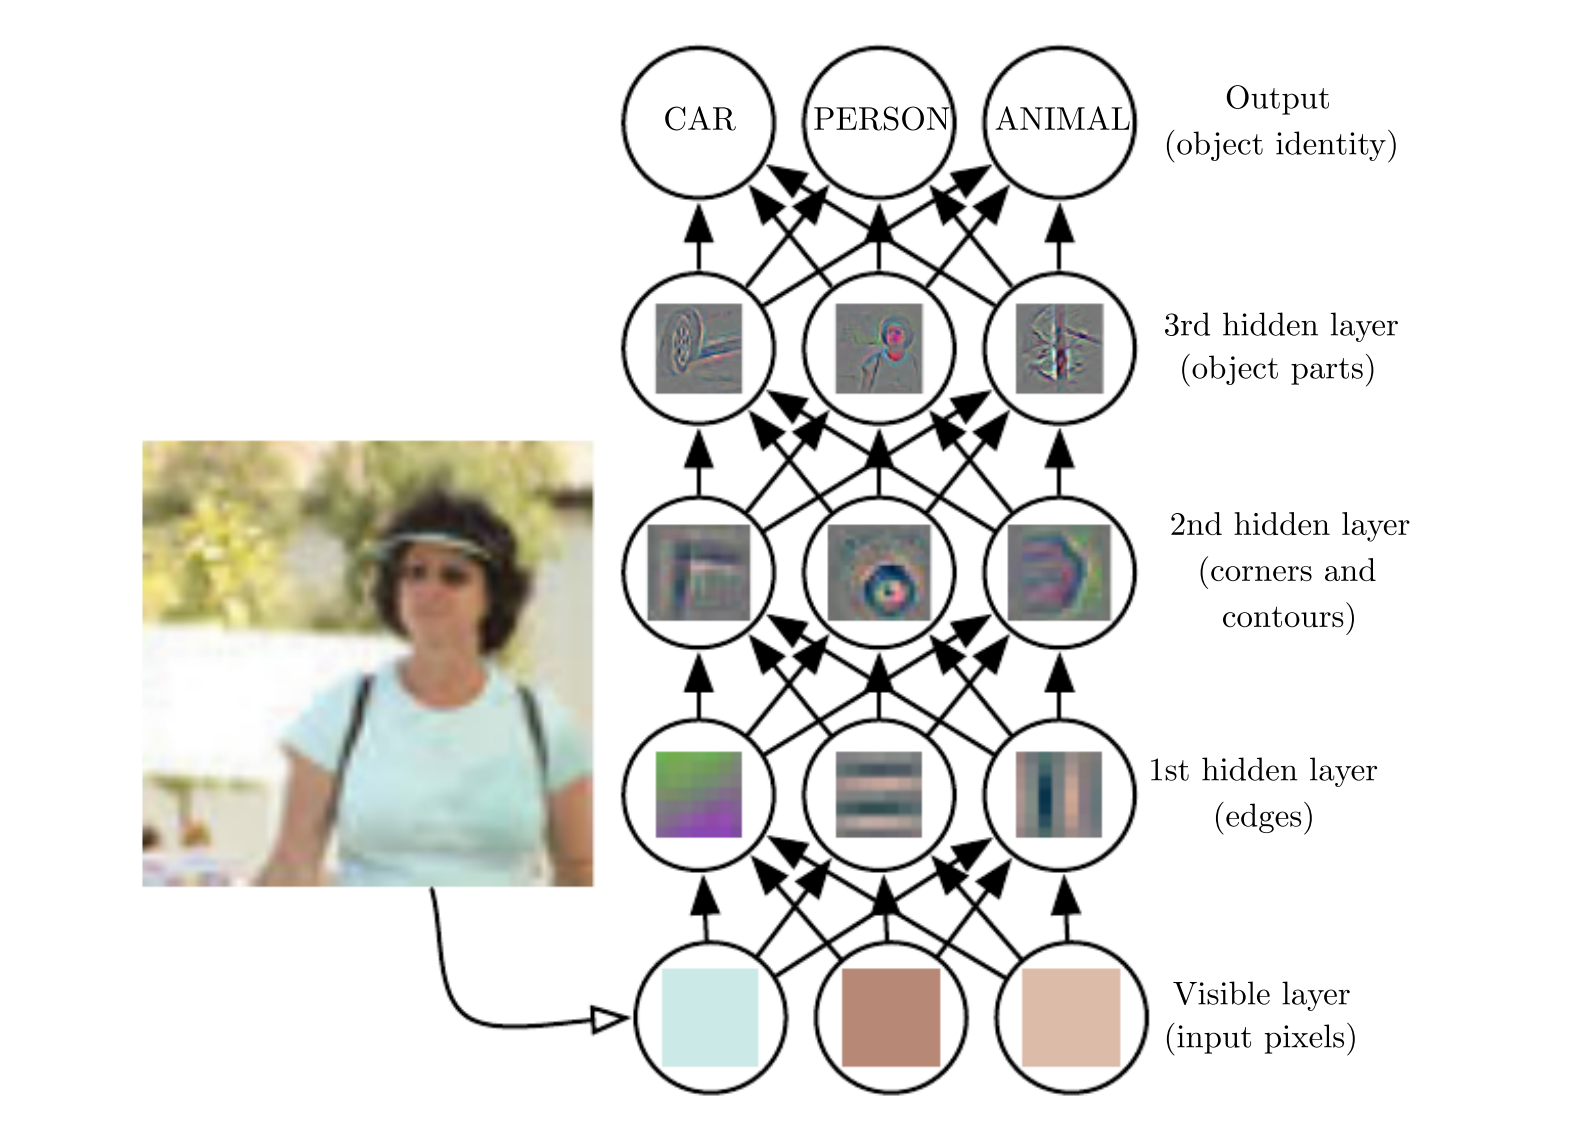
\includegraphics[width=12cm]{kapitel2/vision.png}
  \caption[Illustration eines Deep-Learning-Modells]{Illustration eines Deep-Learning-Modells aus \cite{IanGoodfellowYoshuaBengio2016} und \cite{Suah2017}: Ein Computer kann ohne weiteres das Bild in dieser Abbildung nicht erfassen, da es keine sensorischen Rohdaten verstehen kann. Das Bild in dieser Abbildung ist nur eine Sammlung von Pixelwerten. Die Funktionszuordnung von einem Satz von Pixeln zu einer Objektidentität ist sehr kompliziert.  Deep Learning löst diese Schwierigkeit, indem das gewünschte komplizierte \enquote{Mapping} in eine Reihe verschachtelter einfacher Mappings aufgeteilt wird, die jeweils durch eine andere Ebene des Modells beschrieben werden. Die Eingabe wird auf der \enquote{sichtbaren Ebene} (visible layer) dargestellt. Diese Schicht wird so genannt, weil sie die Variablen enthält, die wir beobachten können. Dann extrahieren eine Reihe \enquote{versteckter Ebenen} (hidden layer) zunehmend abstrakte Merkmale aus dem Bild. Diese Ebenen werden als \enquote{versteckt} bezeichnet, da ihre Werte nicht in den Daten angegeben sind. Stattdessen muss das Modell bestimmen, welche Konzepte zur Erklärung der Beziehungen in den beobachteten Daten nützlich sind. Angesichts der Pixel kann die erste Schicht Kanten nur leicht identifizieren, indem die Helligkeit benachbarter Pixel vergleicht. Angesichts der Beschreibung der Kanten durch die erste verborgene Ebene kann die zweite verborgene Ebene nach Ecken und erweiterten Konturen suchen. Angesichts der Beschreibung des Bildes durch die zweite verborgene Ebene in Bezug auf Ecken und Konturen kann die dritte verborgene Ebene ganze Teile bestimmter Objekte erkennen, indem bestimmte Konturen und Ecken gefunden werden. Schließlich kann diese Beschreibung des Bildes in Bezug auf die darin enthaltenen Objektteile verwendet werden, um die im Bild vorhandenen Objekte zu erkennen.}
  \label{Kap2:Vison}
\end{figure}

\section{Das Perzeptron}
Das Perzeptron kann ins deutsche mit dem Begriff der \enquote{Wahrnehmung} übersetzt werden. Das Perzeptron ist ein einfacher Algorithmus mit einem Eingabevektor $x$ mit $m$ Werten $(x_2, ..., x_m)$. Es wird oft wird als \enquote{Eingabe-Features} oder einfach als \enquote{Features} bezeichnet und zurückgegeben wird entweder eine $1$ \enquote{Ja} oder eine $0$ \enquote{Nein} (siehe Formel~\ref{Formel2_1}).

In Formel~\ref{Formel2_1}  ist $w$ ein Vektor welches das Gewicht darstellt, und $wx$ das Punktprodukt aus $\begin{array}{l}
    {\textstyle \sum ^{m}_{j=1}} w_{j} x_{j} \\
  \end{array}$, $b$ ist der Bias.
Aus $wx + b$ ist die Grenzhyperebene definiert, die die Position gemäß den $w$ und $b$ zugewiesenen Werten ändert.

\begin{equation}
  fx=\begin{cases}
    1 & wx+b >0   \\
    0 & ansonsten
  \end{cases}
  \label{Formel2_1}
\end{equation}

Mit anderen Worten, ist dies ein sehr einfacher, aber effektiver Algorithmus. Beispielsweise kann das Perzeptron bei drei Eingabemerkmalen  (Rot, Grün und Blau) unterscheiden, ob die Farbe weiß ist oder nicht. Es soll beachtet werden, dass das Perzeptron keine \enquote{Vielleicht}-Antwort ausdrücken kann. Es kann mit \enquote{Ja} (1) oder \enquote{Nein} (0) antworten. Das Perzeptron-Modell kann also benutzt werden, indem durch Anpassung von $w$ und $b$, das Modell \enquote{trainiert} wird.


\section{Mehrschichtiges Perzeptron}
In der Vergangenheit war \enquote{Perzeptron} der Name eines Modells mit einer einzigen linearen Schicht. Wenn es mehrere Schichten hat, wurde es daher als mehrschichtiges Perzeptron (Multi-layer perceptron / MLP) bezeichnet. Die Eingabe- und Ausgabeebene  ist von außen sichtbar, während alle anderen Ebenen in der Mitte ausgeblendet sind - daher der Name ausgeblendete Ebenen (hidden layers). In diesem Zusammenhang ist eine einzelne Schicht einfach eine lineare Funktion, und der MLP wird daher erhalten, indem mehrere einzelne Schichten nacheinander gestapelt werden (siehe Abbildung~\ref{Kap2:Multi}).

\begin{figure}[H]
  \centering
  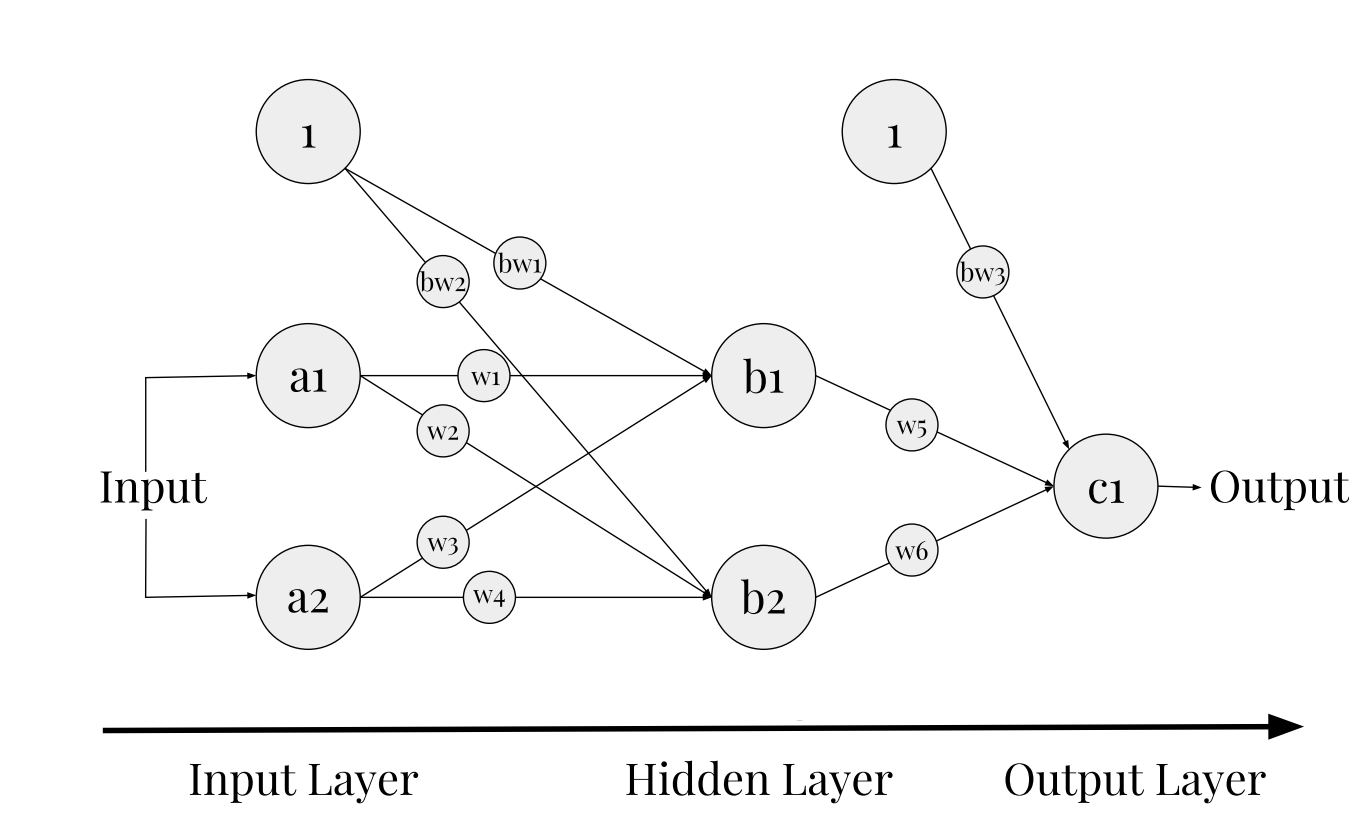
\includegraphics[width=12cm]{kapitel2/multilayer.png}
  \caption[Das mehrschichtige Perzeptron]{Ein Beispiel für ein mehrschichtiges Perzeptron in Anlehnung an \cite{Taylor2017}: Jeder Knoten in der ersten verborgenen Schicht empfängt eine Eingabe und \enquote{feuert} eine 0 oder 1 gemäß den Werten der zugehörigen linearen Funktion. Dann wird die Ausgabe der ersten verborgenen Schicht an die zweite Schicht übergeben, wo eine andere lineare Funktion angewendet wird, deren Ergebnisse an die endgültige Ausgabeschicht übergeben werden. Die letzte Schicht besteht nur aus einem einzelnen Neuron. Es ist interessant festzustellen, dass diese geschichtete Organisation vage der Organisation des menschlichen Sichtsystems ähnelt, wie zuvor besprochen.}
  \label{Kap2:Multi}
\end{figure}

Was sind die besten Entscheidungen für das Gewicht $w$ und den Bias $b$? Um diese Frage zu beantworten, wird nur ein einzelnes Neuron (ein einzelner Knoten) betrachtet.

Im Idealfall werden eine Reihe von Trainingsbeispielen bereitgestellt und der Computer muss das Gewicht $w$ und den Bias $b$ so einstellen, dass die in der Ausgabe erzeugten Fehler minimiert werden.

Um dies etwas konkreter zu machen, wird angenommen, dass es eine Reihe von Katzenbildern vorhanden sind und eine weitere separate Reihe von Bildern, die keine Katzen enthalten. Angenommen, jedes Neuron empfängt Eingaben vom Wert eines einzelnen Pixels in den Bildern. Während der Computer diese Bilder verarbeitet, möchten wir, dass unser Neuron seine Gewichte und seine Vorspannung so anpasst, dass immer weniger Bilder falsch erkannt werden.
Dieser Ansatz scheint sehr intuitiv zu sein, erfordert jedoch eine kleine Änderung der Gewichte (oder des Bias), um nur eine kleine Änderung der Ausgänge zu bewirken. Wenn wir einen großen Leistungssprung haben, können wir nicht progressiv lernen. Es wird gewünscht, wie ein \enquote{Kind} zu lernen, nach und nach. Das Perzeptron zeigt jedoch dieses \enquote{Stück für Stück}-Verhalten nicht. Ein Perzeptron gibt entweder eine 0 oder eine 1 zurück und das ist ein großer Sprung, der beim Lernen nicht hilft.


\section{Sigmoid-Neuron}
Das Verhalten des Perzeptron ist sehr  \enquote{uneben}, sodass ein \enquote{glatteres} nötig ist. Wir brauchen eine Funktion, die sich ohne Diskontinuität schrittweise von 0 auf 1 ändert. Mathematisch bedeutet dies, dass wir eine stetige Funktion benötigen, mit der wir die Ableitung berechnen können.

Dieses Problem kann überwunden werden, indem einen neuer Typ eines künstlichen Neurons eingeführt wird, der als Sigmoid-Neuron. Sigmoidneuronen ähneln Perzeptronen, sind jedoch so modifiziert, dass kleine Änderungen ihres Gewichts und ihres Bias nur eine geringe Änderung ihrer Leistung bewirken. Dies ist die entscheidende Tatsache, die es einem Netzwerk von Sigmoidneuronen ermöglicht, zu lernen \cite*[S. 8]{Nielsen}.

Genau wie ein Perzeptron hat das Sigmoid-Neuron die Eingaben $x_1, x_2, ...$, aber anstatt nur 0 oder 1 zu sein, können diese Eingänge auch beliebige Werte zwischen 0 und 1 annehmen. Also zum Beispiel 0,123 welches eine gültige Eingabe für ein Sigmoid-Neuron ist. Ebenso wie ein Perzeptron hat das Sigmoid-Neuron Gewichte für jede Eingabe, $w_1, w_2, ...$ und einen Bias, $b$. Die Ausgabe ist jedoch nicht 0 oder 1, stattdessen ist es $\sigma$, $(wx + b)$, wobei $\sigma$ als Sigmoidfunktion bezeichnet wird und durch Formel~\ref{Formel2_2} definiert ist.

\begin{equation} \label{Formel2_2}
  \sigma (z) = \frac{1}{1+e^{-z}}
\end{equation}


\section{Aktivierungsfunktionen}
Ohne eine Aktivierungsfunktion (auch als Nichtlinearität bezeichnet) würde die dichte Schicht (dense layer) nuraus zwei linearen Operationen bestehen - einem Punktprodukt und einer Addition: $Ausgabe = Punkt (w, Eingabe) + b$. Die Schicht konnte also nur lineare Transformationen (affine Transformationen) der Eingabedaten lernen. Um Zugang zu einem viel umfangreicheren Hypothesenraum zu erhalten, wird eine Nichtlinearitäts- oder Aktivierungsfunktion benötigt \cite*[S. 72]{Chollet2017}. Es gibt weitaus mehr Aktivierungsfunktionen, als die in die in diesem Abschnitt beschriebenen. Es sollen hier nur die gängigsten 3 vorgestellt werden.

\subsection{Sigmoid}
Die Sigmoidfunktion wurde bereits mit der Formel~\ref{Formel2_2} definiert und in der Abbildung~\ref{Kap2:Sigmoid_plot} dargestellt. Sie hat kleine Ausgangsänderungen im Bereich (0, 1), wenn der Eingang im Bereich $(-\infty, \infty)$ variiert. Mathematisch ist die Funktion stetig. Ein Neuron kann das Sigmoid zur Berechnung der nichtlinearen Funktion $\sigma(z = wx + b)$ verwenden.
Wenn $z = wx + b$ sehr groß und positiv ist, dann wird $e^z \rightarrow 0$ also $\sigma(z) \rightarrow 1$, während wenn $z = wx + b$ sehr groß und negativ ist dann wird $e^{-z} \rightarrow 0$ also $\sigma(z) \rightarrow 0$. Mit anderen Worten, ein Neuron mit Sigmoidaktivierung hat ein ähnliches Verhalten wie das Perzeptron, aber die Änderungen sind allmählich und Ausgabewerte wie 0,54321 oder 0,12345 sind vollkommen legitim. In diesem Sinne kann ein Sigmoid-Neuron \enquote{vielleicht} antworten \cite*[S. 10]{AntonioGuili;AmitaKapoor;SujitPal2019}.
\begin{figure}[H]
  \centering
  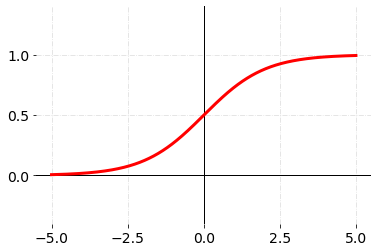
\includegraphics[width=8cm]{kapitel2/sig_plot.png}
  \caption[Darstellung der Sigmoid-Aktivierungsfunktion]{Darstellung der Sigmoid-Aktivierungsfunktion (eigene Darstellung)}
  \label{Kap2:Sigmoid_plot}
\end{figure}

\subsection{Tanh}
Die Tanh-Aktivierungsfunktion wird mit der Formel~\ref{Formel2_3} definiert. Sie hat ihre Ausgangsänderungen im Bereich (-1, 1). Sie hat eine Struktur, die der Sigmoid-Funktion sehr ähnlich ist. Der Vorteil gegenüber der Sigmoidfunktion besteht darin, dass ihre Ableitung steiler ist, was bedeutet, dass sie mehr Wert erhalten kann (vergleiche Abbildung~\ref{Kap2:Tanh_plot}).

\begin{equation} \label{Formel2_3}
  tanh(z) = \frac{e^{z}-e^{-z}}{e^{z}-e^{-z}}
\end{equation}

\begin{figure}[H]
  \centering
  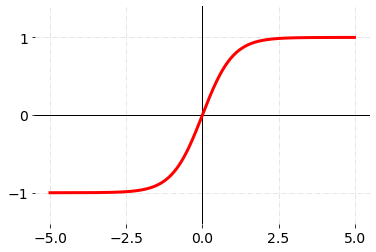
\includegraphics[width=8cm]{kapitel2/tanh_plot.png}
  \caption[Darstellung der Tanh-Aktivierungsfunktion]{Darstellung der Tanh-Aktivierungsfunktion (eigene Darstellung)}
  \label{Kap2:Tanh_plot}
\end{figure}

\subsection{ReLu}
Vor kurzem wurde eine sehr einfache Funktion namens ReLU (REctified Linear Unit) sehr beliebt, da sie dazu beiträgt, einige bei Sigmoiden beobachtete Optimierungsprobleme zu lösen \cite*[S. 11]{AntonioGuili;AmitaKapoor;SujitPal2019}. Eine ReLU wird relativ einfach in und wird in der Formel~\ref{Formel2_4} definiert. Wie in Abbildung~\ref{Kap2:ReLu_plot} zu sehen, ist die Funktion für negative Werte Null und wächst für positive Werte linear. Die ReLU ist auch sehr einfach zu implementieren (im Allgemeinen reichen drei Anweisungen aus), während das Sigmoid einige Größenordnungen mehr benötigt.

\begin{equation} \label{Formel2_4}
  f( x) \ =\ \begin{cases}
    0 & \textrm{\textit{für}}\ x < \ 0   \\
    x & \textrm{\textit{für}}\ x\geq \ 0
  \end{cases}
\end{equation}

\begin{figure}[H]
  \centering
  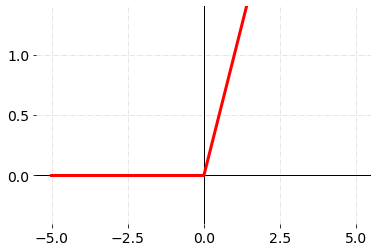
\includegraphics[width=8cm]{kapitel2/relu_plot.png}
  \caption[Darstellung der ReLu-Aktivierungsfunktion]{Darstellung der ReLu-Aktivierungsfunktion (eigene Darstellung)}
  \label{Kap2:ReLu_plot}
\end{figure}




\section{Verlustfunktion und Kreuzentropie}
Innerhalb eines neuronalen Netzwerks wandelt eine Verlustfunktion alle möglichen Fehler, in eine Zahl um, die den Gesamtfehler des Netzwerks darstellt. Im Wesentlichen ist es ein Maß dafür, wie falsch ein Netzwerk ist. Auf einer technischeren Ebene werden ein Ereignis oder Werte einer oder mehrerer Variablen einer reellen Zahl zugeordnet. Diese reelle Zahl stellt  den \enquote{Verlust} oder die \enquote{Kosten} dar, die mit dem Ereignis oder den Werten verbunden sind \cite*[S. 41]{Taylor2017}.

\subsection{Mittlere quadratische Abweichung}
Wie der Name sagt, wird mit der mittleren quadratischen Abweichung (MSE), der Verlust berechnet, indem der Mittelwert der quadratischen Differenzen zwischen tatsächlichen Ziel- und vorhergesagten Werten genommen wird. Sie wird in Formel~\ref{Formel2_5} definiert.

\begin{equation} \label{Formel2_5}
  MSE\ =\frac{1}{n}{\displaystyle \sum ^{n}_{i=1}( d-y)^2}
\end{equation}

Diese Funktion ist der Durchschnitt aller Fehler, die in jeder Vorhersage gemacht wurden. Wenn eine Vorhersage weit vom wahren Wert entfernt ist, wird dieser Abstand durch die \enquote{Quadrierungsoperation} deutlicher. Außerdem kann das Quadrat den Fehler addieren, unabhängig davon, ob ein bestimmter Wert positiv oder negativ ist \cite*[17]{AntonioGuili;AmitaKapoor;SujitPal2019}.

Grundsätzlich kann diese Verlustfunktion verwendet werden, wenn die Ausgabe eine reelle Zahl ist. Die MSE-Verlustfunktion wird meistens für Regressionsaufgaben verwendet.

\subsection{Binäre Kreuzentropie}
\subsection{Kategoriale Kreuzentropie}


% \section{Formelsatz}

% Eine Formel gefällig? Mitten im Text $a_2 = \sqrt{x^3}$ oder als eigener Absatz (siehe Formel~\ref{Formel}):




% Das Aufkommen von Online-Nachrichtenagenturen und die Explosion der Anzahl der Benutzer, die Nachrichten mit diesem Medium konsumieren, haben dazu geführt, dass mehrere Webseiten miteinander konkurrieren, um die Aufmerksamkeit der Benutzer zu erregen. Dies hat dazu geführt, dass Verkaufsstellen kreative Wege geschaffen haben, um Leser auf ihre Website zu locken. Eine der am häufigsten verwendeten Techniken ist die Verwendung von Clickbait-Überschriften. Diese Überschriften wurden speziell dafür entwickelt, um das Interesse des Lesers an dem zu wecken, was versprochen wird. Wenn auf den Artikel geklickt wird jedoch, liefert dieser Artikel normalerweise nicht den Inhalt, den der Leser Ursprüngich gesucht hat. In den Abbildungen \ref{Kap2:ClickBait} und \ref{Kap2:News}\footnote{Entnommen aus: https://github.com/MichaelGoodale/Clickbait-Classifier} wird der Unterschied zwischen Clickbaits und \enquote{normalen} Nachrichten aufgezeigt.

% \begin{figure}
%   \centering
%   \includegraphics[width=12cm]{kapitel2/clickbait.png}
%   \caption[Beispiel von Clickbait]{Beispiel von Clickbait}
%   \label{Kap2:ClickBait}
% \end{figure}


% \begin{figure}[ht]
%   \centering
%   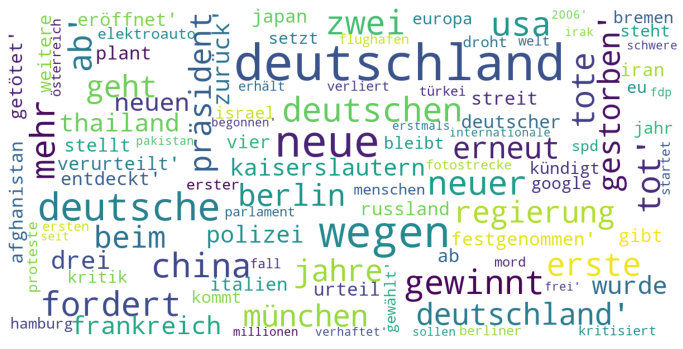
\includegraphics[width=12cm]{kapitel2/news.png}
%   \caption[Beispiel von \enquote{normalen} Nachrichten]{Beispiel von \enquote{normalen} Nachrichten}
%   \label{Kap2:News}
% \end{figure}


% \section{Lösungsansatz}
% Textklassifizierung ist eine gängige Art, wie man \enquote{gute} von \enquote{bösen} Texten unterscheiden kann. Es ist allerdingt nicht praktisch ein großes Sprachmodell wie GPT-3 Browserkompatible zu machen. Erstens ist es völlig \enquote{overkill} für ein solches Problem ein Sprachmodell zu benutzen und zweitens passen diese großen Modelle nicht in den Browser, da die Ladezeit nicht praktisch ist.

% Mit dieser Arbeit möchte ich ein Modell erstellen, um Clickbait Überschriften zu erkennen. Es wäre Hilfreich, wenn es ein Dienst gibt, welches eine Überschrift liest und dem Benutzer vorhersagt, ob es sich um Clickbait handelt oder nicht. So kann der Nutzer seine Zeit sparen und muss nicht auf die Seite gehen. Das Hauptprodukt ist dabei dieser Dienst, welches ganz einfach in jede HTML-Seite importiert werden kann. Dieser Dienst muss klein und schnell und gute dabei möglichst Ergebnisse liefern.

% \section{Aufbau der Arbeit}


% Im Abschnitt 2.6 Grobgliederung befindet sich eine mögliche Gliederung für diese Arbeit, auf die ich verweisen möchte. Zunächst wird in den Kapiteln 2 und 3 eine theoretische Grundlage geschaffen. Diese Kapitel beschäftigen sich mit Deep Learning und den mathematisch/statistschischen Erklärungen. Kapitel 3 orientiert sich eher mit NLP und insbesondere mit Worteinbettungen und wie moderne Computer die natürliche Sprache verstehen. Kapitel 4 soll den aktuellen Forschungsstand mit meiner Arbeit vergleichen. Es sollen verwandte Lösungsansätze kategorisch analysiert werden.

% Um mit dem eigentlichen Kern anzufangen, benötigt diese Arbeit an Daten. In Kapitel 5 wird gezeigt wie mittelt Webscraping. Dieser Datensatz wird händisch gelabelt und besteht aus einem Titel und einer Klasse. Die erste erste hälfte des Datensatzes wird aus Wikinews\footnote{https://de.wikinews.org/wiki/Hauptseite} geladen. Wikinews hat einen API-Zugang wodurch Nachrichten, welche nicht Clickbait sind in den Datensatz gebracht werden können. Ich habe dafür bereits mehr als 10.000 Nachrichten-Titel in eine Datenbank geladen. Die zweite hälfte des Datensatzes wird mittels Webseiten mit Scrapy\footnote{ https://scrapy.org/} gescraped. Die ersten 1.000 Titel sind bereits in die Datenbank\footnote{https://github.com/youurt/klickkoeder/blob/main/klickscraper/klickscraper.db} geladen worden.

% Nachdem ausreichend Daten geladen werden, ist geplant diese Daten zu laben. Damit später keine Verzerrungen bei den Daten entstehen, plane ich noch eine weitere Person zum Unterstützen beim Labeln mit in die Arbeit zu nehmen. Dieses wird mit dem Betreuer der Arbeit noch abgeklärt werden müssen. Der restliche Teil dieses Kapitels beschäftigt sich mit der Analyse der Daten um bestimmte Muster zu erkennen und die Daten in ein passendes Format zu bringen.

% Ich werde ein Modell in TensorFlow.js entwickeln. Dieses Modell soll möglichst klein sein und schnell sein. Um mit TensorFlow.js arbeiten zu können muss der Text in Vektoren umgewandelt werden.

% Mit einem Versuchsaufbau soll das Modell getestet und analysiert werden. Schließlich soll das Modell in die Browser-Umgebung gebracht und mittels eines minimalistischen React Frontends angeboten werden.

% \begin{figure}[ht]
%   \centering
%   \includegraphics[width=12cm]{kapitel2/beispiel.png}
%   \caption[Beispiel einer Systemarchitektur]{Beispiel einer Systemarchitektur entnommen aus \cite{cho2019shop}. Der Client bekommt beim laden der Seite, neben dem HTML, CSS und dem JavaScript, welches für das Frontend nötig ist, ein weiteres Script, welches die TensorFlow.js API bereitstellt. Die Berechnung findet im Browser, beim Client statt, wo auch das Modell sich befindet.}
%   \label{Kap2:SystemArchitektur}
% \end{figure}

% \section{Wissenschaftlicher Beitrag}
% \begin{itemize}
%   \item Den Stand der Technik in Bezug auf Deep Learning und Worteinbettungen zeigen
%   \item Erstellung und labeln eines Datensatzes für deutsche Clickbaits
%   \item Implementierung eines NLP-Problemes im Browser ohne zusätzliche Software oder Plugins, mit TensorFlow.js
%   \item Optimierung des Browsers für Deep Learning
%   \item Auswahl des optimalen Modells und der Trainingsmethode
%   \item Produktion eines Dienstes, um Clickbait Nachrichten vorzubeugen
% \end{itemize}

% \section{Einstiegsliteratur}

% \begin{itemize}
%   \item \cite{Kaur2020a}
%   \item \cite{Chavan2019}
%   \item \cite{vorakitphan2018clickbait}
%   \item \cite{Anand2017}
%   \item \cite{gairola2017neural}
%   \item \cite{kumar2018identifying}
%   \item \cite{glenski2017fishing}
%   \item \cite{chawda2019novel}
%   \item \cite{seopredicting}
%   \item \cite{cho2019shop}
%   \item \cite{roberts2018magenta}
%   \item \cite{aggarwal2012survey}
%   \item \cite{kowsari2019text}
%   \item \cite{korde2012text}
%   \item \cite{altinel2018semantic}
%   \item \cite{nordberg2020crucial}
%   \item \cite{raamkumar2020use}
%   \item \cite{rivera2020identifying}
%   \item \cite{nguyen2020real}
%   \item \cite{zhang2015character}
%   \item \cite{kiranyaz20191d}
%   \item \cite{severyn2015unitn}
%   \item \cite{severyn2015twitter}
%   \item \cite{zhao2019speech}
%   \item \cite{eren2019generic}
% \end{itemize}

% \section{Grobgliederung}
% \renewcommand{\labelenumii}{\theenumii}
% \renewcommand{\theenumii}{\theenumi.\arabic{enumii}.}

% \begin{enumerate}

%   \item Einleitung
%         \begin{enumerate}
%           \item Motivation
%           \item Wissenschaftlicher Beitrag
%           \item Struktur der Arbeit
%         \end{enumerate}

%   \item Neuronale Netze
%         \begin{enumerate}
%           \item Einleitung
%           \item Arten des Neuronalen Lernens
%           \item Netzwerkparameter und Hyperparameter
%           \item Aktivierungsfunktionen
%           \item Verlustfunktion
%           \item Optimizer
%           \item Epochen
%           \item TensorFlow.js
%           \item Schluss
%         \end{enumerate}

%   \item Die natürliche Sprache
%         \begin{enumerate}
%           \item Einleitung
%           \item Vektorisierung des Textes durch Encoding
%           \item Worteinbettungen
%           \item 1d CNN
%           \item Schluss
%         \end{enumerate}

%   \item Aktueller Forschungsstand
%         \begin{enumerate}
%           \item Einleitung
%           \item Clickbaits und Deep Learning Ansätze
%           \item TensorFlow.js
%           \item Worteinbettungen
%         \end{enumerate}

%   \item Korpuskonstruktion und Analyse
%         \begin{enumerate}
%           \item Einleitung
%           \item Rohdatenerhebung mittels Webscraping
%           \item Das labeln der Daten
%           \item Explorative Datenanalyse
%           \item Vorverarbeitung der Daten
%           \item Schluss
%         \end{enumerate}

%   \item Methodik
%         \begin{enumerate}
%           \item Einleitung
%           \item Die Systemarchitektur
%           \item JavaScript
%           \item Modelling
%           \item Einbettung in das Frontend
%           \item Schluss
%         \end{enumerate}

%   \item Versuchsaufbau und Diskussion der Ergebnisse
%         \begin{enumerate}
%           \item Einleitung
%           \item Anpassung der Netzwerkparameter und Hyperparameter
%           \item Leistungsmessungen
%           \item Vergleich und Darstellung der Ergebnisse
%           \item Schluss
%         \end{enumerate}

%   \item Schluss
%         \begin{enumerate}
%           \item Fazit zum Forschungsbeitrag
%           \item Abschließende Gedanken
%           \item Zukunft der Arbeit
%         \end{enumerate}
% \end{enumerate}




% \section{Hervorhebungen}
% \label{Einleitung:Textauszeichnungen}

% Achten Sie bitte auf die grundlegenden Regeln der Typographie\index{Typographie}\footnote{Ein Ratgeber in allen Detailfragen ist \cite{Forssman2002}.}, wenn Sie Ihren Text schreiben. Hierzu gehören z.\,B. die Verwendung der richtigen "`Anführungszeichen"' und der Unterschied zwischen Binde- (-), Gedankenstrich (--) und langem Strich (---). Sie erhalten den Bindestrich in \LaTeX{} mit \verb+-+, den Gedankenstrich mit \verb+--+ und den langen Strich mit \verb+---+.

% Wenn Sie Text hervorheben wollen, dann setzten Sie ihn mit \verb+\textit+ \textit{kursiv} (Italic) und nicht \textbf{fett} (Bold). Fettdruck ist Überschriften vorbehalten; im Fließtext stört er den Lesefluss. Das \underline{Unterstreichen} von Fließtext ist im gesamten Dokument tabu und kann maximal bei Pseudo"=Code vorkommen.\index{Hervorhebungen}


% \section{Anführungszeichen}

% Deutsche Anführungszeichen werden mit \verb+"`+ und \verb+"'+ erzeugt: "`dieser Text steht in \glq Anführungszeichen\grq; alles klar?"'. Englische Anführungszeichen hingegen mit \verb+``+ und \verb+''+: ``this is an `English' quotation''. Beachten Sie, dass Sie in Zitaten immer die zur Sprache passenden Anführungszeichen verwenden. Die Verwendung von \verb+"+ ist für Anführungszeichen immer falsch und führt bei \LaTeX{} zu seltsamen "Effekten".

% Um sich diesen Ärger zu sparen, biete sich die Verwendung des Paketes \textit{csquotes} und des Kommandos \verb+\enquote+ an. Hierdurch werden die Anführungszeichen korrekt für die eingestellte Sprache gesetzt und Sie müssen sich \enquote{keine Sorgen mehr über die \enquote{Anführungszeichen} machen}.


% \section{Abkürzungen}
% \index{Abkürzungen}
% \index{Abbreviation|see{Abkürzungen}}

% Eine \ac{ABK} (\verb+\ac{ABK}+) wird bei der ersten Verwendung ausgeschrieben. Danach nicht mehr: \ac{ABK}. Man kann allerdings mit \verb+\acl+ die Langform explizit anfordern (\acl{ABK}) oder mit \verb+\acs+ die Kurzform (\acs{ABK}) oder mit \verb+\acf+ auch noch einmal die Definition (\acf{ABK}).

% Beachten Sie, dass bei Abkürzungen, die für zwei Wörter stehen, ein kleines Leerzeichen nach dem Punkt kommt: z.\,B. bzw. \zb{} und d.\,h. bzw. \dahe{}. Das Template bietet hierfür die beiden Makros \verb+\zb{}+ und \verb+\dahe{}+.


% \section{Querverweise}

% Querverweise auf eine Kapitelnummer macht man im Text mit \verb+\ref+ (Kapitel~\ref{Einleitung:Textauszeichnungen}) und auf eine bestimmte Seite mit \verb+\pageref+ (Seite~\pageref{Einleitung:Textauszeichnungen}). Man kann auch den Befehl \verb+\autoref+ benutzen, der automatisch die Art des referenzierten Elements bestimmt (\zb{} \autoref{Einleitung:Textauszeichnungen} oder \autoref{Kap2:Kopplungsformen}).


% \section{Fußnoten}

% Fußnoten werden einfach mit in den Text geschrieben und zwar genau an die Stelle\footnote{An der die Fußnote auftauchen soll}. Hierzu dient der Befehl \verb+\footnote{Text}+.


% \section{Tabellen}

% Tabellen werden normalerweise ohne vertikale Striche gesetzt, sondern die Spalten werden durch einen entsprechenden Abstand voneinander getrennt.\footnote{Siehe \cite[S. 89]{Willberg1999}.} Zum Einsatz kommen ausschließlich horizontale Linien (siehe Tabelle~\ref{Kap2:Kopplungsformen}).

% \begin{table}[h]
%   \caption{Ebenen der Kopplung und Beispiele für enge und lose Kopplung}
%   \label{Kap2:Kopplungsformen}
%   \renewcommand{\arraystretch}{1.2}
%   \centering
%   \sffamily
%   \begin{footnotesize}
%     \begin{tabular}{l l l}
%     \toprule
%     \textbf{Form der Kopplung} & \textbf{enge Kopplung} & \textbf{lose Kopplung}\\
%     \midrule
%     Physikalische Verbindung	&	Punkt-zu-Punkt	& 	über Vermittler\\
%     Kommunikationsstil	&	synchron		&	asynchron\\
%     Datenmodell	&	komplexe gemeinsame Typen	&	nur einfache gemeinsame Typen\\
%     Bindung	&	statisch		&	dynamisch\\
%     \bottomrule
%     \end{tabular}
%   \end{footnotesize}
%   \rmfamily
% \end{table}

% Eine Tabelle fließt genauso, wie auch Bilder durch den Text. Siehe Tabelle~\ref{Kap2:Kopplungsformen}.

% Manchmal möchte man Tabellen, in denen der Text in der Tabellenspalte umbricht. Hierzu dient die Umgebung \texttt{tabularx}, wobei \texttt{L} eine Spalte mit Flattersatz und \texttt{X} eine mit Blocksatz definiert. Die Breite der Tabelle kann über den Faktor vor \verb+\textwidth+ angegeben werden.

% \begin{table}[h]
%   \caption{Teildisziplinen der Informatik}
%   \label{Kap2:Teildisziplinen}
%   \renewcommand{\arraystretch}{1.2}
%   \centering
%   \sffamily
%   \begin{footnotesize}
%     \begin{tabularx}{0.9\textwidth}{l X L}
%       \toprule
%       \textbf{Gebiet} & \textbf{Definition} & \textbf{Beispiel}\\
%       \midrule
%       \emph{Praktische Informatik} & Informatik-Disziplinen, welche sich vorwiegend mit der Entwicklung und Anwendung der Software-Komponenten befassen & Programmentwicklung, Compilerbau; im Aufbau von z.B. Informationssystemen und Netzwerken ergeben sich Überlappungen mit der technischen Informatik \\
%       \emph{Technische Informatik} & Informatik-Disziplinen, welche sich vorwiegend mit der Entwicklung und Anwendung der Hardware-Komponenten befassen & Digitaltechnik, Mikroprozessortechnik \\
%       \emph{Theoretische Informatik} & Informatik-Disziplinen, welche sich mit der Entwicklung von Theorien und Modellen der Informatik befassen und dabei viel Substanz aus der Mathematik konsumieren & Relationenmodell, Objekt-Paradigmen, Komplexitätstheorie, Kalküle \\
%       \emph{Angewandte Informatik} & Informatik als instrumentale Wissenschaft & Rechtsinformatik, Wirtschaftsinformatik, Geoinformatik \\
%       \bottomrule
%     \end{tabularx}
%   \end{footnotesize}
%   \rmfamily
% \end{table}


% \section{Harveyballs}

% \begin{quote}
%     Harvey Balls sind kreisförmige Ideogramme, die dazu dienen, qualitative Daten anschaulich zu machen. Sie werden in Vergleichstabellen verwendet, um anzuzeigen, inwieweit ein Untersuchungsobjekt sich mit definierten Vergleichskriterien deckt. \parencite{Wikipedia_HarveyBalls}
% \end{quote}

% \begin{table}[h]
%   \caption{Beispiel für Harvey Balls}
%   \label{tab:harveyexample}
%   \centering
%   \begin{tabular}{lccc}
%     \toprule
%     & Ansatz 1 & Ansatz 2 & Ansatz 3\\
%     \midrule
%     Eigenschaft 1	& \harveyBallNone & \harveyBallQuarter & \harveyBallHalf \\
%     Eigenschaft 2	& \harveyBallHalf & \harveyBallThreeQuarter & \harveyBallFull \\
%     Eigenschaft 3	& \harveyBallFull & \harveyBallThreeQuarter & \harveyBallQuarter\\
%     \bottomrule
%   \end{tabular}
% \end{table}


% \section{Aufzählungen}

% Aufzählungen sind toll.

% \begin{itemize}
%   \item Ein wichtiger Punkt
%   \item Noch ein wichtiger Punkt
%   \item Ein Punkt mit Unterpunkten
%     \begin{itemize}
%       \item Unterpunkt 1
%       \item Unterpunkt 2
%     \end{itemize}
%   \item Ein abschließender Punkt ohne Unterpunkte
% \end{itemize}


% Aufzählungen mit laufenden Nummern sind auch toll.

% \begin{enumerate}
%   \item Ein wichtiger Punkt
%   \item Noch ein wichtiger Punkt
%   \item Ein Punkt mit Unterpunkten
%     \begin{enumerate}
%       \item Unterpunkt 1
%       \item Unterpunkt 2
%     \end{enumerate}
%   \item Ein abschließender Punkt ohne Unterpunkte
% \end{enumerate}
